\chapter{Design}
\label{chapter3}
This chapter will outline the proposed design of the cloud gaming system as well as the game that will be used to run on the system. Also at a high level, I will discuss the virtual network design that will be used to simulate a cloud data center as well as the proposed solution to use software-defined networking to reduce latency in the network.

\section{Cloud Gaming System}
As a result of the background research conducted, the cloud gaming system will aim to offload the game engine to the cloud data center. This includes the game logic, physics and graphics rendering. Due to this, it will leave the client's application to just take control of receiving physical button input and send this to the game server as well as receiving and displaying the game video frames.
\newline
\par
It can be seen at Figure \ref{fig:cloudmodel} that multiple players should be able to connect to the cloud server and a new virtual machine should be generated for each player. For each virtual machine, an instance of the game will be executed with the required resources such as RAM and processing power provided by the cloud's resource manager. The resources required can be specified as a template with the parameters already set. This makes sure that each game instance has sufficient resources to run at smoothly.
\newline
\par
A design improvement on this is to allow the client to specify the video settings to use such as 1080p resolution at 60 fames-per-second and 720p resolution at 30 frames-per-second. Enabling this option will give the client an option to manually improve their gameplay experience since sending higher resolution frames as well as more of them per second will require higher bandwidth. This also helps the cloud data centre to use different templates for virtual machine resources so they will not be wasted by providing too much and therefore can be allocated to other virtual machines.
\newline
\par
The software-defined networking controller will manage the networking inside the data centre. It will have global knowledge of the all switches and the links between them. A load balancing application will be used to make sure that traffic generated with the video streaming is routed appropriately to help keep latency in the network to a minimum. This will be discussed later on section 3.4.
\clearpage
\begin{figure}[h]
 \centering
 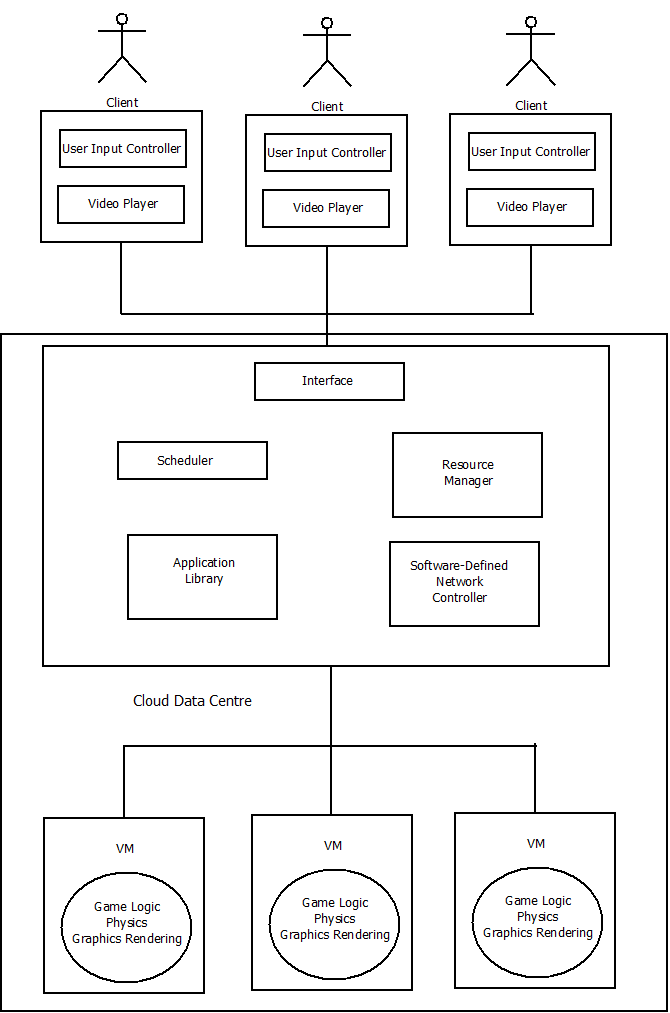
\includegraphics[width=0.8\linewidth]{images/cloudsystemmodel.png}
 \caption{Cloud Gaming System Model}
 \label{fig:cloudmodel}
\end{figure}

\section{Game Design}
In this section I will indicate the design of the game at a high level that will developed to be used as the program to benchmark on the cloud gaming system. The aim of this game is to be somewhat computationally expensive to warrant as a program that will improve by being on a system that is more powerful than a mainstream consumer system. The game should be configurable so it can test out the limits of the system by increasing the amount of computer power it needs. It should also implement a method to measure latency that will arise not just numerically but through user input and immediate visual feedback. The client will experience this lag when a button is pressed, but the expected visual feedback is not being displayed as soon as expected.
\newline
\par
To make the game computationally challenging, trees will be modelled and generated in real time. Plants and trees are part of the natural environment and are often used in games to create a realistic scenery. They are geometrically complex and difficult to generate realistic models in real time. Such trees are usually pre-generated and saved locally so it can be loaded easily when needed, but this means the game is limited to using those models and tree models will have to be repeated. This degrades the player's experience as they see duplicate trees in the scenery reminding them that they are in a game which breaks the immersion.
\newline
\par
Lindenmayer systems or 'L-systems' is a part of formal language theory to write parallel grammars describing growth similar to the way DNA is a programming language of the human body \cite{prusinkiewicz2012algorithmic}. Plants tend to have patterns in their growth, but fundamentally they grow forward, rotate then branch out in a hierarchy starting from the root. L-systems are stated as production rules and correspond to each stage of growth for each part of the plant according to a fixed pattern. The notation in the pattern can be simplified to:
\begin{itemize}
 \item F 	:	move forward and draw
 \item +,- \(\theta\)	:	rotate \(\theta\) around x-axis
 \item \&,\(\wedge\) \(\theta\)	:	rotate \(\theta\) around y-axis
 \item /,\(\backslash\) \(\theta\)	:	rotate \(\theta\) around z-axis
 \item {[,]}	:	push / pop
\end{itemize}

\[Trunk \rightarrow F[+\theta /\theta Branch][-\theta \backslash\theta Branch]\]
\[Branch \rightarrow F[+\theta /\theta Branch][-\theta \backslash\theta Branch]\]

\section{Virtual Network}
\lipsum[1-1]

\section{SDN Application Design}
\lipsum[1-1]